\documentclass[a4paper]{article}
\author{
\includegraphics[width=0.2\textwidth]{images/logo_fundacio.png}
}
\title{\textbf{Manual d'usuari \emph{fiberfy-nt}}}

\usepackage{xcolor}
\usepackage{float}
\usepackage{graphicx}
\usepackage{titlesec}
\usepackage{subcaption}
\usepackage{setspace}
\usepackage{hyperref}
\usepackage[utf8]{inputenc}
\usepackage[catalan]{babel}

\definecolor{mygreen}{rgb}{0,0.6,0}
\definecolor{mygray}{rgb}{0.5,0.5,0.5}
\definecolor{mymauve}{rgb}{0.58,0,0.82}

\date{11 d'octubre de 2018}
\titleformat{\section}
{\normalfont\fontsize{16}{18}\bfseries}{\thesection}{1em}{}

\titlespacing*{\section}
{0pt}{5.5ex plus 1ex minus .2ex}{4.3ex plus .2ex}
\titlespacing*{\subsection}
{0pt}{5.5ex plus 1ex minus .2ex}{4.3ex plus .2ex}
\titlespacing*{\subsubsection}
{0pt}{5.5ex plus 1ex minus .2ex}{1.3ex plus .2ex}

\addtolength{\oddsidemargin}{-.875in}
\addtolength{\evensidemargin}{-.875in}
\addtolength{\textwidth}{1.75in}
\addtolength{\topmargin}{-.875in}
\addtolength{\textheight}{1.75in}

\begin{document}
	\maketitle
	\newpage
	
	\begin{center}
		\begin{tabular}{| p{1.89cm} | p{2.21cm} | p{8.42cm} |} \hline
			\multicolumn{3}{|c|}{\large{\textbf{Historial de versions}}} \\ \hline
			\textbf{Versió} & \textbf{Data} & \textbf{Canvis} \\ \hline
			prototip & 10/08/2017 & Primera edició del document. Versió antiga del fiberfy \\ \hline
			18.10 & 11/10/2018 & Primera versió estable de l'aplicació. Canvis rellevants:
			\begin{itemize}
				\item El frontend canvia el nom a fiberfy-nt
				\item Es refà per complet l'aplicació només mantenint els mapes
				\item S'incorpora un importador de projectes
				\item S'incorpora un nou tipus de localització: No Definit
				\item Es demana confirmació al eliminar entitats
				\item S'incorpora un buscador de projectes
			\end{itemize} \\ \hline
		\end{tabular}
	\end{center}
	\newpage
	\tableofcontents
	\newpage
	\onehalfspacing
	
	\section{Introducció}
	L'eina de desplegaments de fibra òptica \emph{fiberfy-nt} ha estat creada per facilitar la confecció de projectes als diferents operadors de la xarxa \textbf{Guifi.net}.
	Aquest document és manual d'usuari per ensenyar les característiques de l'aplicació i explicar-ne el seu funcionament. 
	
	\section{Accés al portal}
	L'aplicació \emph{fiberfy-nt} és un servei web accessible des de qualsevol dipositiu amb un navegador compatible amb \textbf{JavaScript}. La seva direcció és: \url{https://fiberfy.guifi.net/}
	
	\begin{figure}[H]
		\centering
		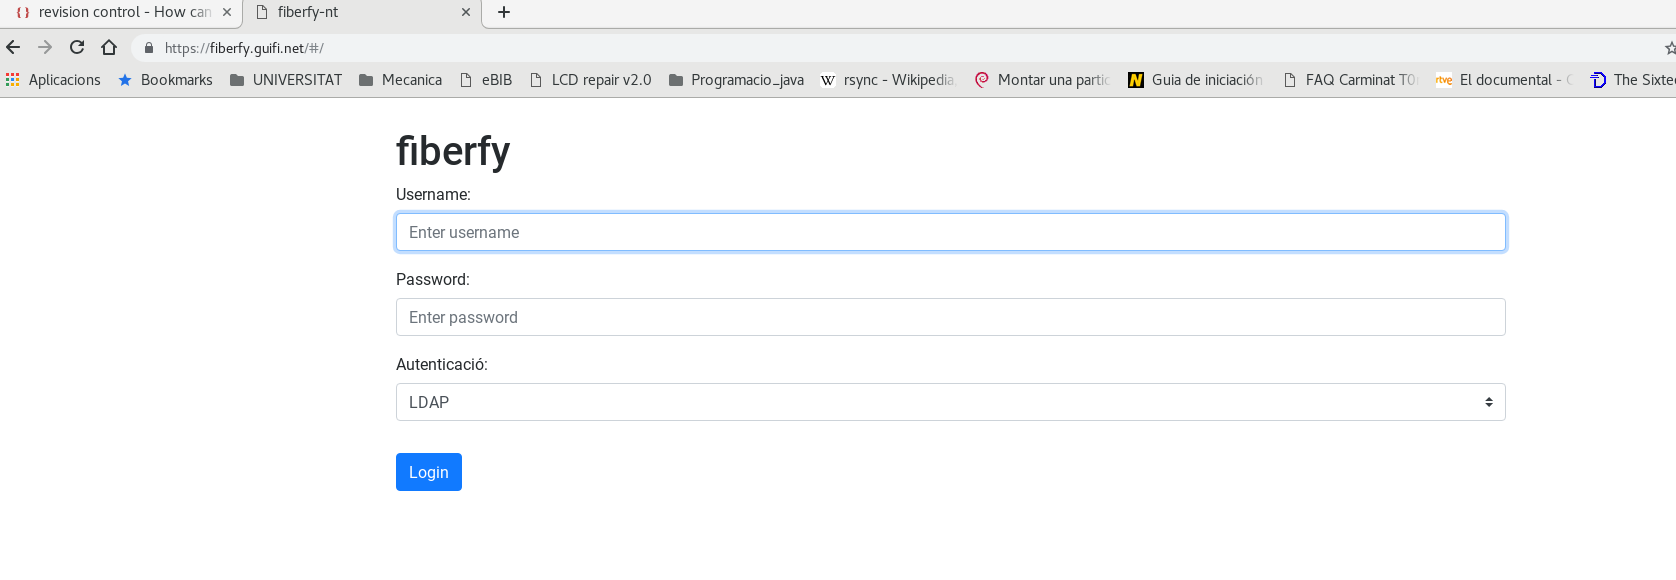
\includegraphics[width=0.7\textwidth]{images/login_screen.png}
		\caption{Pantalla de login \emph{fiberfy-nt}}
	\end{figure}

	Els paràmetres d'accés vindran subministrats per la fundació. Actualment es pot autenticar usuaris mitjançant l'\textbf{LDAP} del \textbf{GLIR}, per tant l'usuari podrà usar el mateix usuari pels diferents serveis que s'ofereixen. Un cop l'usuari s'ha autenticat li apareixerà un mapa de Catalunya.
	
	\begin{figure}[H]
		\centering
		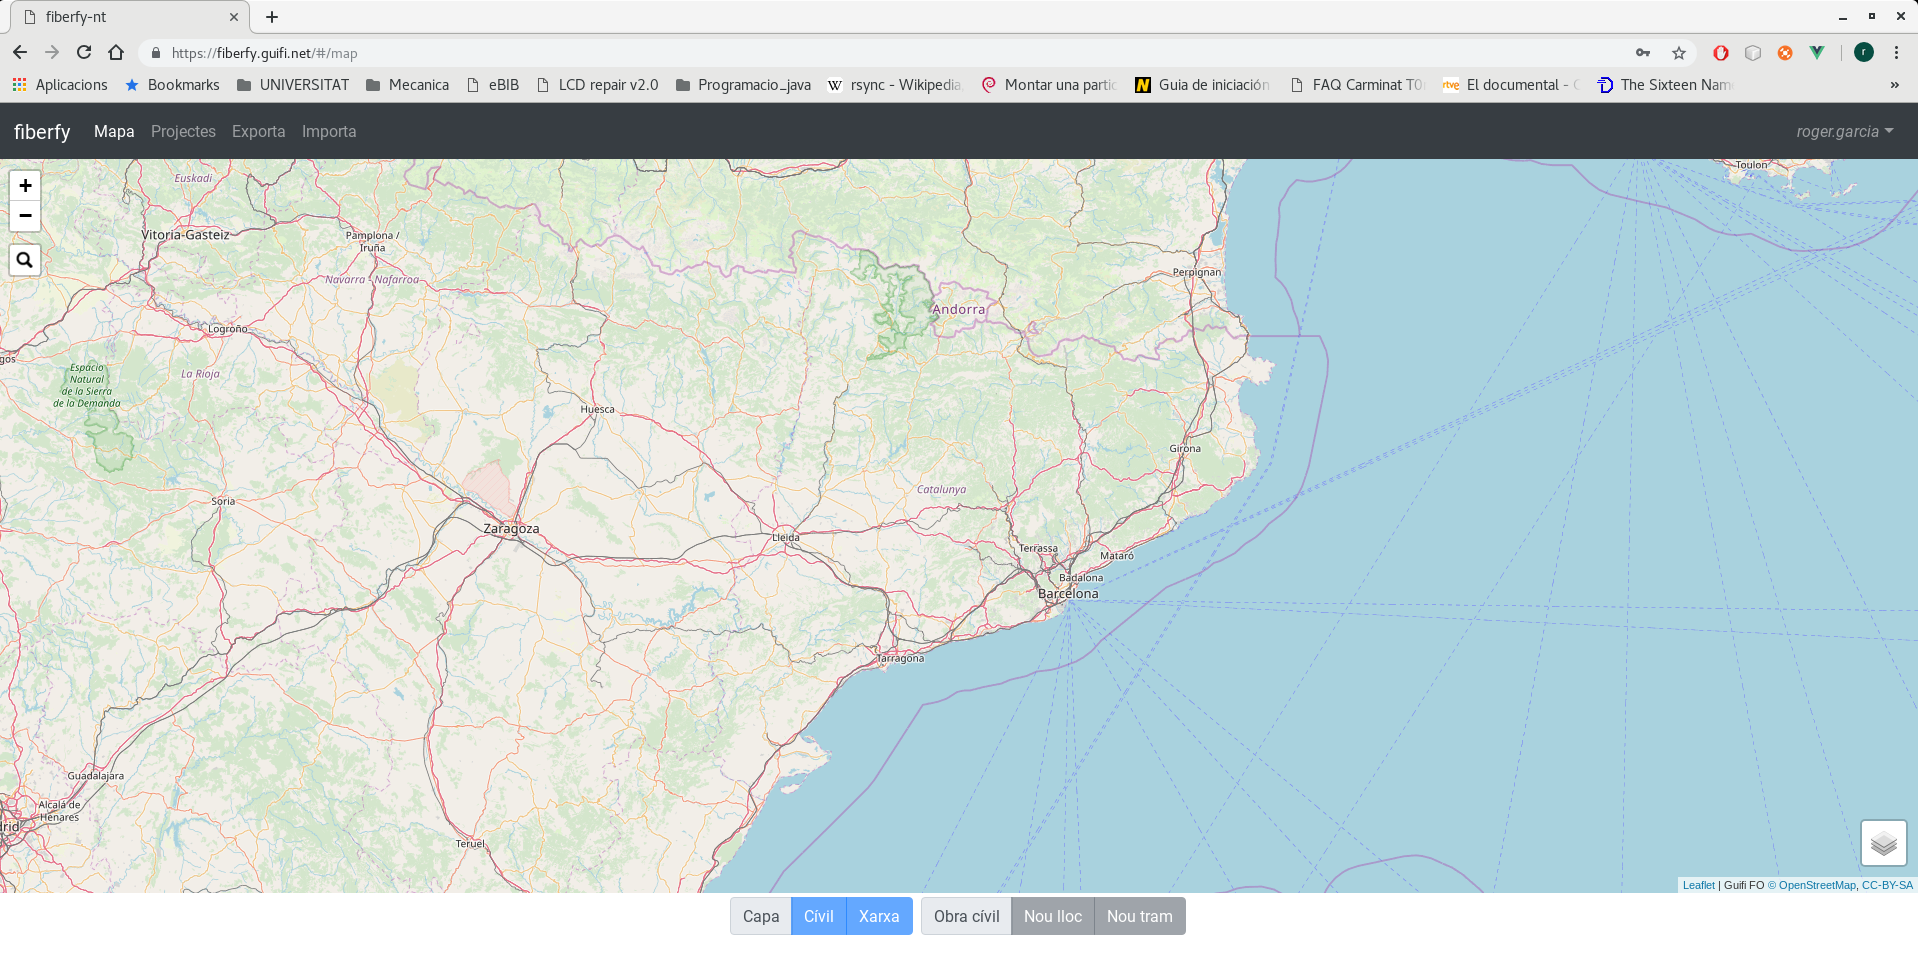
\includegraphics[width=0.7\textwidth]{images/map_screen.png}
		\caption{Mapa d'inici \emph{fiberfy-nt}}
	\end{figure}

	\section{Funcionament del mapa}
	El mapa ens permet treballar amb diferents capes. Hi ha dos tipus de capes:
	\begin{itemize}
		\item Capes base: Aquestes són les capes bàsiques que ens gràfiquen l'esquelet del mapa; només s'en pot seleccionar una a la vegada. A dia d'avui tenim la capa gratuïta d'\textbf{OpenStreetMap} i diverses capes de \textbf{Google}.
		\item Capes auxiliars: Aquestes són capes que es mostren a sobre de la capa base i ens aporten informació extra. Actualment disposem de 4 capes de Guifi.net (nodes, enllaços, localitzacions (fibra), \emph{trams} (fibra).
	\end{itemize}
	Per interactuar amb les diferents capes del mapa situarem el punter sobre un pictograma situat al extrem inferior dret com podem veure a la figura \ref{fig:pictogram-layer}:
	
	\begin{figure}[H]
		\centering
		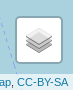
\includegraphics{images/pictogram_layer.png}
		\caption{Pictograma gestió de capes}
		\label{fig:pictogram-layer}
	\end{figure}

	A la figura \ref{fig:layer-manager} podem veure el gestor de capes del mapa.
	\begin{figure}[H]
		\centering
		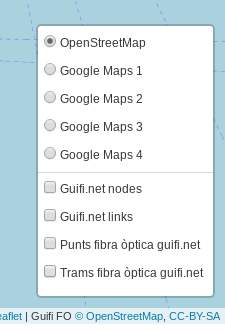
\includegraphics{images/layer_manager.png}
		\caption{Menú de gestió de capes}
		\label{fig:layer-manager}
	\end{figure}
	
	\section{Gestió de projectes}
	Per tal de crear projectes haurem d'accedir al menú situat a la capçalera de la pàgina i accedirem a la pestanya de projectes.
	
	\begin{figure}[H]
		\centering
		
\includegraphics{images/topbar_menu_1.png}
		\caption{Menú superior \emph{fiberfy-nt}}
	\end{figure}
	Al formulari de projectes ens apareixerà primer una petita targeta amb la informació del projecte seleccionat que ens permetrà modificar les seves característiques:
	\begin{itemize}
		\item \emph{Guardar Posició}: Aquest botó ens guarda la posició del mapa actual al projecte. Així quan tornem a utilitzar l'aplicació ens mantindrà aquesta posició i no haurem de navegar pel mapa buscant-lo.
		\item \emph{Editar}: Aquest botó ens porta a un formulari on podrem modificar els atributs del projecte
	\end{itemize}
	Ens apareixerà un buscador de projectes i a la part inferior es mostraran els resultats obtinguts. Per defecte es mostren tots els projectes; si l'usuari desitja mostrar tots els projectes després d'haver fet una búsqueda haurà d'esborrar el text i tornar a prémer \textbf{Buscar}.
	Els projectes de cada usuari seran visibles per tots els usuaris i només podran ser modificats per ell mateix. Per tal de treballar sobre qualsevol projecte aquest s'haurà d'activar prement el botó \emph{Activar} situat a la barra de botons de la dreta.
	
	\begin{figure}[H]
		\centering
		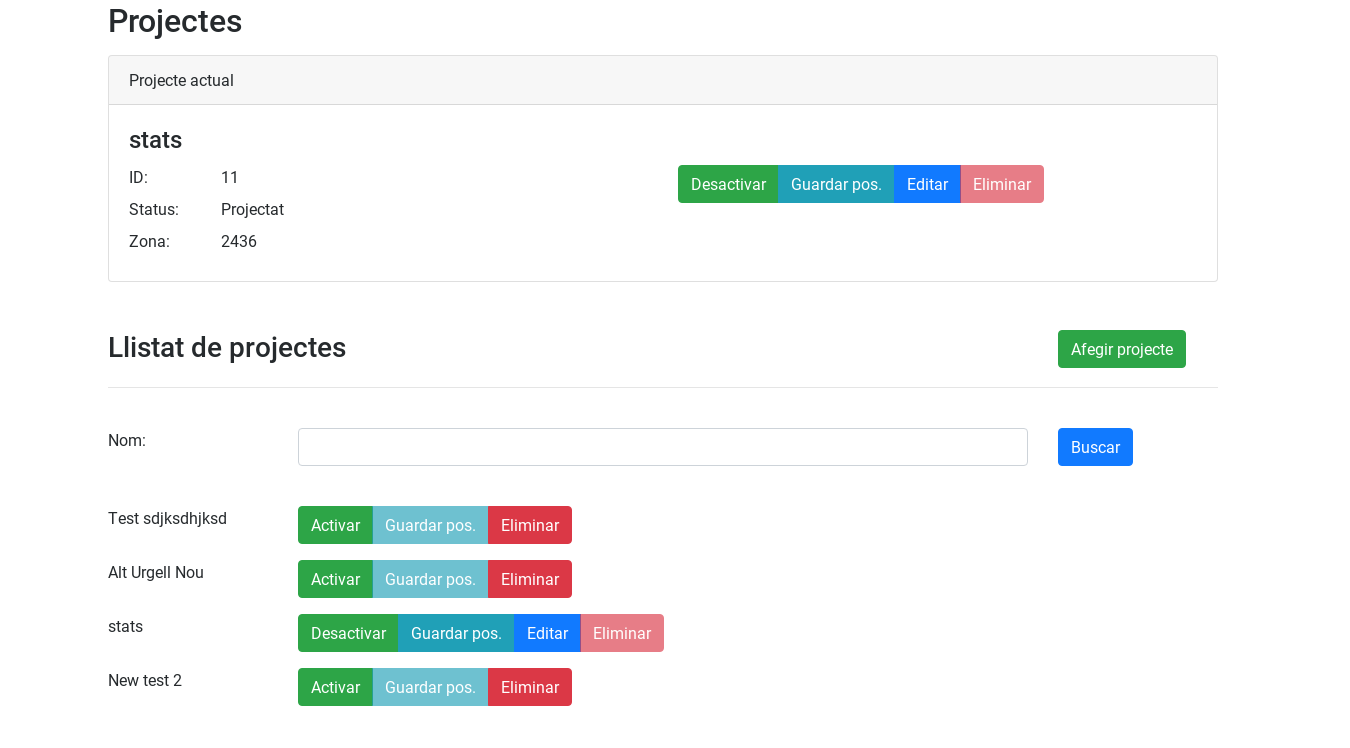
\includegraphics[width=0.8\textwidth]{images/projects_form.png}
		\caption{Formulari de projectes \emph{fiberfy-nt}}
	\end{figure}

	Per tal de crear nous projectes haurem de prémer el botó verd \textbf{Nou projecte} situat a la part superior dreta del Llistat de projectes.
	
	\subsection{Edició}
	Per tal d'editar projectes l'usuari haurà de prémer el botó blau \emph{Editar} i serà conduït a un formulari com el que podem veure a la següent figura:
	
	\begin{figure}[H]
		\centering
		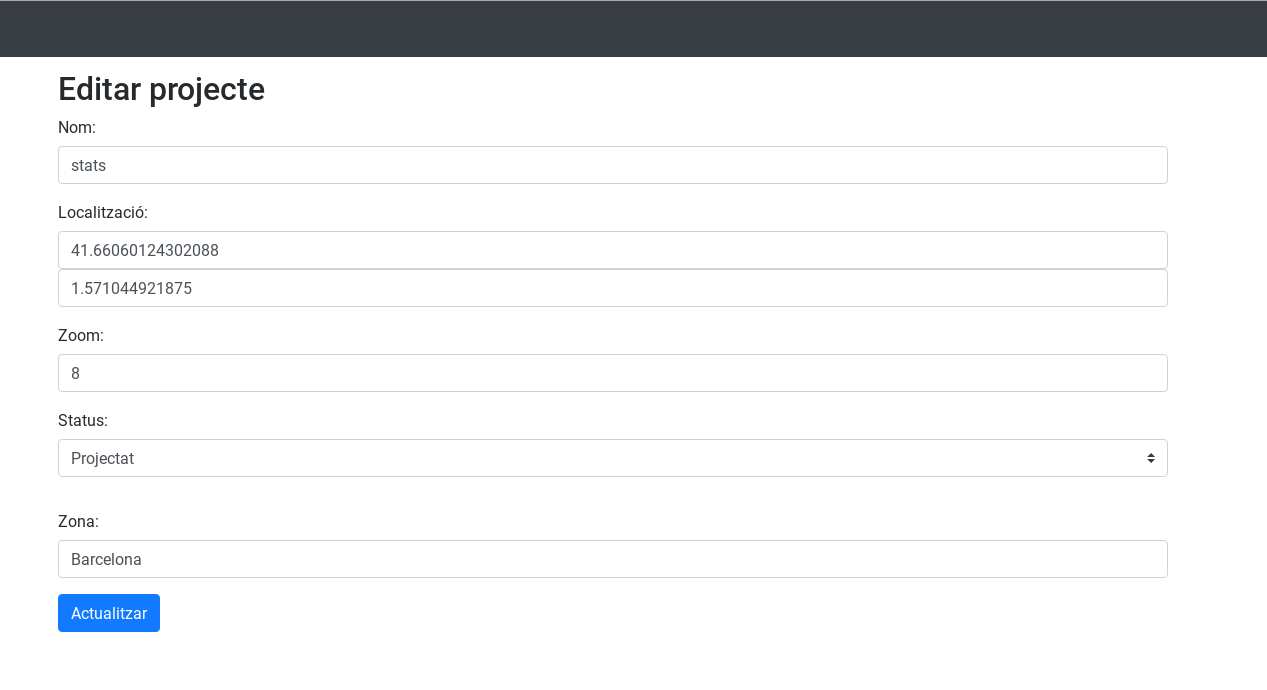
\includegraphics[width=0.8\textwidth]{images/project_edit_form.png}
		\caption{Formulari de projectes \emph{fiberfy-nt}}
	\end{figure}

	Aquí l'usuari podrà modificar aspectes com el nom del projecte, el punt de referència del mapa (Localització + zoom), status (el mateix que hi ha a la web de Guifi.net) i finalment la zona per defecte. La zona ve donada per la base de dades de Guifi.net (la mateixa que la web), l'usuari la pot seleccionar d'un desplegable a mesura que va escrivint.
	
	\newpage
	\section{Obra civil}
	\subsection{Importador}
	Una de les novetats més importants del \emph{fiberfy-nt} és la possibilitat d'importar mapes existents de punts i línies i tractar-los com si de localitzacions i trams es tractessin. Per tal d'importar informació necessitem haver creat prèviament un projecte i tenir-lo activat. Un cop cumplim aquest requisit podem accedir a la pestanya d'\emph{Importa} i podrem veure un formulari com el següent:
	
	\begin{figure}[H]
		\centering
		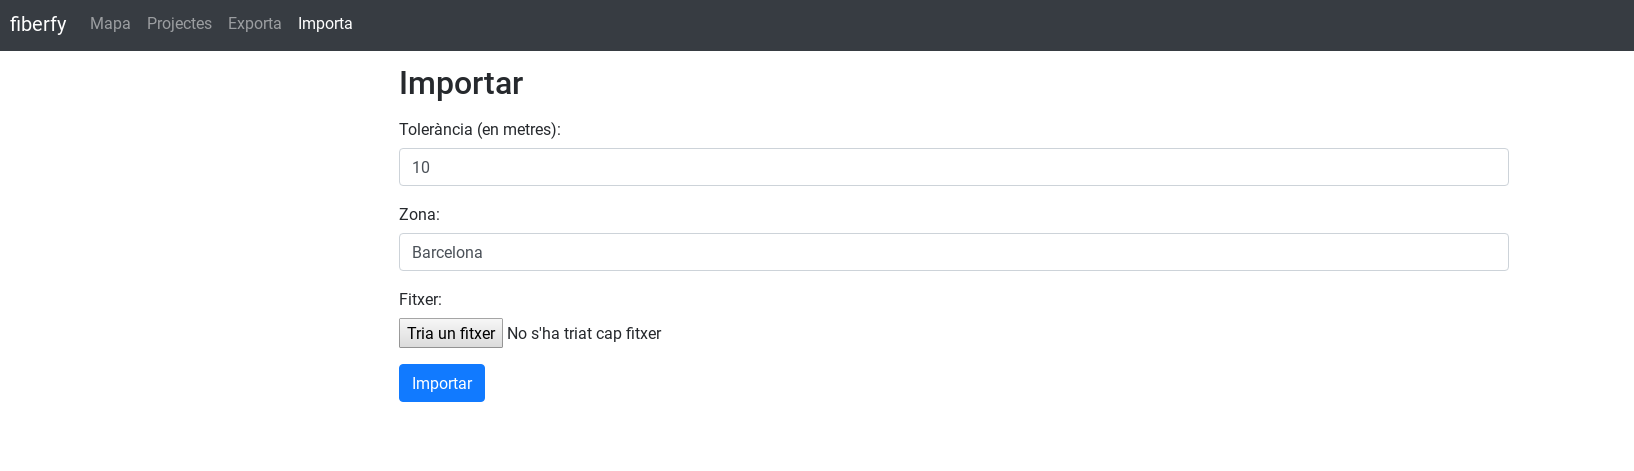
\includegraphics[width=0.8\textwidth]{images/import_form.png}
		\caption{Formulari d'importació d'obra civil}
		\label{fig:import-form}
	\end{figure}

	La tolerància és el marge que té l'algoritme per unir trams amb llocs. Els estàndards de \textbf{GIS} no contemplen la possibilitat d'acoplar punts i rectes, per tant a l'hora d'establir els enllaços l'aplicació els ha de predir. El marge de tolerància indica en metres la distància màxima d'unió de rectes en un únic punt.
	La zona és la mateixa que s'introduiria al crear un node de Guifi (per defecte la del projecte).
	Finalment hem de seleccionar el fitxer que volem importar. Els formats suportats són:
	\begin{itemize}
		\item \textbf{KML}
		\item \textbf{KMZ}
		\item \textbf{GeoJSON}
	\end{itemize}
	
	En cas de disposar d'altres formats es poden convertir a qualsevol dels compatibles. Igualment sempre hi ha la possibilitat d'obrir un \emph{ticket} per tal de resoldre qualsevol incidència.
	
	\subsection{Exportador}
	Aquesta funcionalitat ens permet exportar tota l'obra civil d'un projecte en el format \textbf{GeoJSON}. Per tal de fer-ho servir necessitem haver seleccionat un projecte prèviament i accedir a la pestanya \emph{Exporta}. Aleshores ens apareixerà un formulari amb un botó per descarregar el fitxer:
	
	\begin{figure}[H]
		\centering
		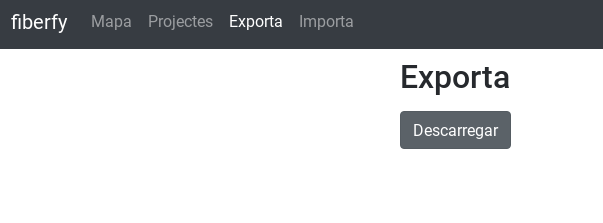
\includegraphics[width=0.8\textwidth]{images/export_form.png}
		\caption{Formulari d'exportació d'obra civil}
		\label{fig:export-form}
	\end{figure}
	
	\subsection{Gestió de llocs}
	Els llocs dins de l'aplicació simbolitzen els punts físics d'obra civil on s'ubicaran les caixes i sistemes de telecomunicacions. Contenen unes coordenades i atribut físic que ens indica el tipus d'element. També permeten afegir comentaris i modificar-ne el nom.
	
	\subsubsection{Creació}
	Sobre el mapa inicial podem crear diferents llocs on s'ubicaran els equips de fibra òptica. Per tal de crear nous llocs hem de seleccionar el botó \emph{Nou lloc} situat a la barra inferior dreta\footnote{És necessari seleccionar la capa d'Obra Cívil}. Aleshores hem d'anar marcant amb el botó esquerre del ratolí els punts on hi volem col·locar un nou \emph{lloc}. Per sortir del menú de creació de nous llocs podem clicar un altre cop sobre el botó \emph{Nou \emph{lloc}} o prémer la fletxa enrere verda.
	
	\begin{figure}[H]
		\centering
		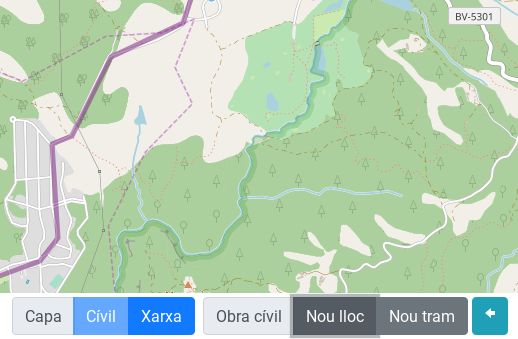
\includegraphics[width=0.7\textwidth]{images/newsite_menu.png}
		\caption{Menú de creació llocs}
		\label{fig:newsite-menu}
	\end{figure}
	
	% Aquí s'ha d'afegir una llegenda dels símbols
	Els llocs creats se simbolitzaran amb els següents marcadors:
	\begin{figure}[H]
		\centering
		\begin{tabular}{|c|p{5cm}|} \hline
			\textbf{Símbol} & \textbf{Explicació} \\ \hline
			
\includegraphics{images/simbols/notdefined.png} & Símbol no definit, quan no coneixem el tipus. \\ \hline
			
\includegraphics{images/simbols/manhole.png} & Arqueta situada al sòl. \\ \hline
			
\includegraphics{images/simbols/pole.png} & Poste \\ \hline
			
\includegraphics{images/simbols/hook.png} & Ganxo \\ \hline
			
\includegraphics{images/simbols/poe.png} & Poe \\ \hline
			
\includegraphics{images/simbols/cabinet.png} & Armari \\ \hline
			
\includegraphics{images/simbols/room.png} & Cambra \\ \hline
			
\includegraphics{images/simbols/jump.png} & Salt \\ \hline
		\end{tabular}
	\end{figure}
	
	Per defecte tots els llocs creats seran de tipus \textbf{No Definit}.
	
	\begin{figure}[H]
		\centering
		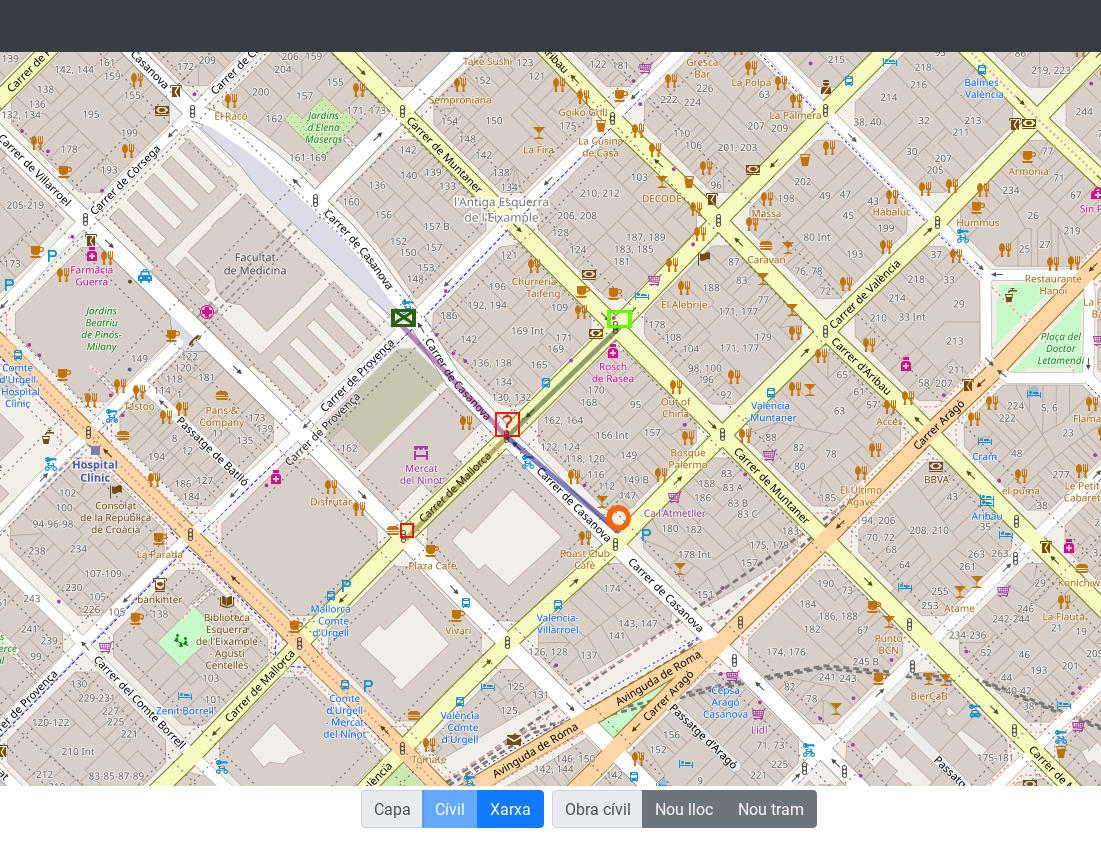
\includegraphics[width=0.8\textwidth]{images/sites_map.png}
		\caption{Mapa amb llocs}
	\end{figure}

	\subsubsection{Edició}
	Per editar un \emph{lloc} des de la capa d'\emph{Obra Civil} hem de clicar sobre el \emph{lloc} del mapa que volem modificar. Aleshores s'ens projectarà un formulari amb tots els atributs rellevants pel \emph{lloc}. Els atributs modificables són: les coordenades, el nom, el tipus de \emph{lloc}, observacions i l'estatus en que es troba. També ens mostrarà la distància en metres que cobreix.
	
	\begin{figure}[H]
		\centering
		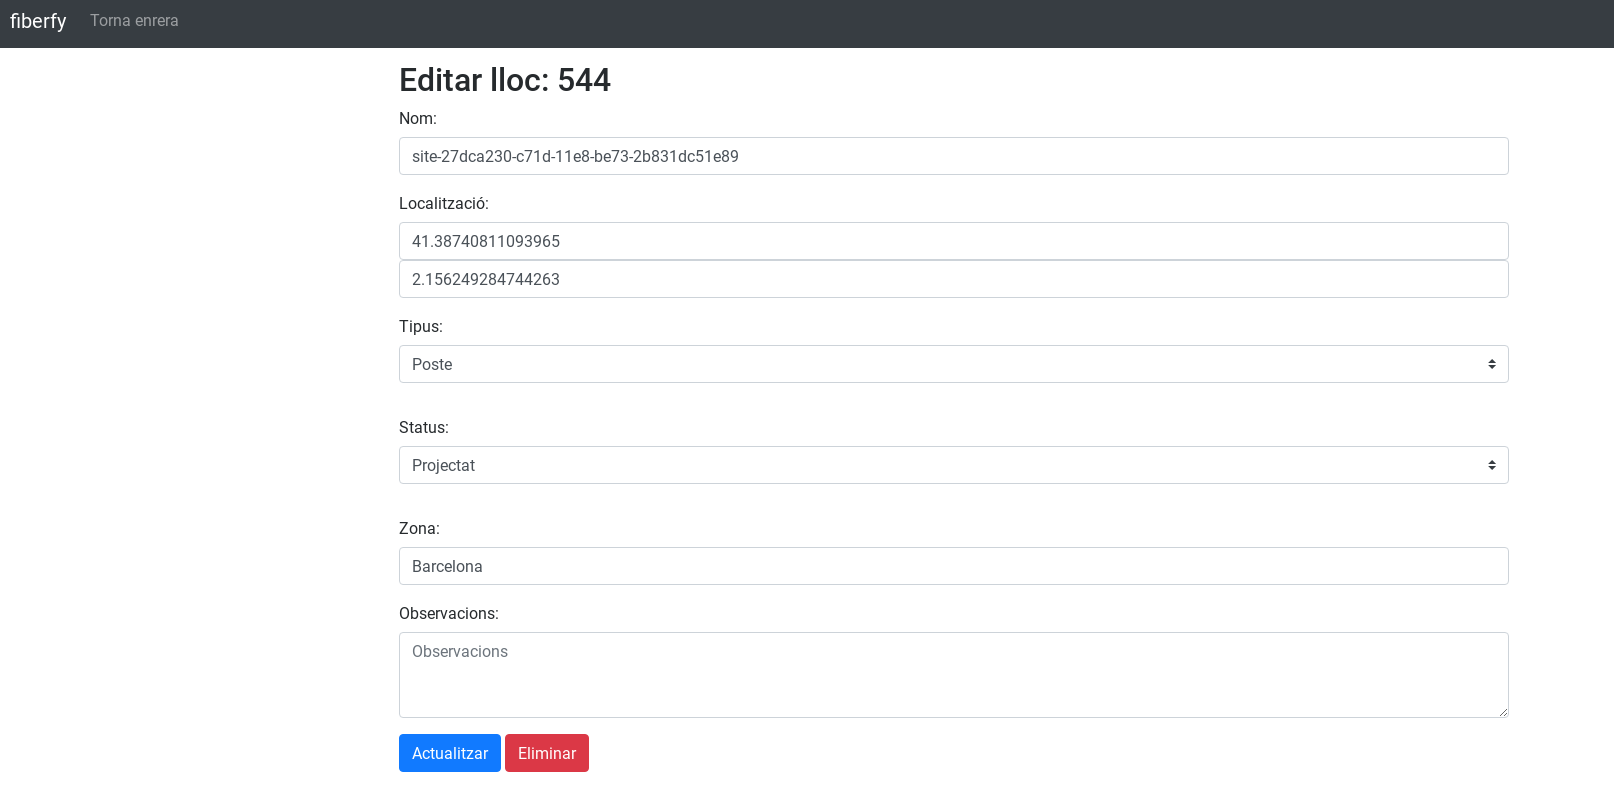
\includegraphics[width=0.8\textwidth]{images/sites_edit.png}
		\caption{Formulari d'edició de llocs}
	\end{figure}

	Si hem realitzat qualsevol modificació que volem guardar abans de tornar al mapa haurem de clicar el botó \emph{Actualitzar}.
	
	Si volem eliminar el \emph{lloc} haurem de clicar el botó \emph{Eliminar}; aleshores s'ens demanarà confirmació i en cas afirmatiu eliminarà el \emph{lloc} i ens redirigirà al mapa.
	
	\subsection{Gestió de \emph{trams}}
	Els \emph{trams} dins de l'aplicació ens indicaran l'obra civil encarregada d'unir uns determinats llocs. Podrem definir com serà aquest tram i escriure alguna anotació(observació).
	
	\subsubsection{Creació}
	Per tal de crear \emph{trams} haurem de seleccionar el botó \emph{Crea Tram} del menú d'Obra Civil\footnote{És necessari seleccionar la capa d'Obra Cívil}. Un cop seleccionat el botó hem de clicar sobre el primer \emph{lloc} que volem unir i anar clicant sobre els següents llocs adjacents tot traçant una línia.
	
	En cas de voler desfer la creació del tram només hem de prémer el botó verd amb la fletxa enrera.
	
	
	\begin{figure}[H]
		\centering
		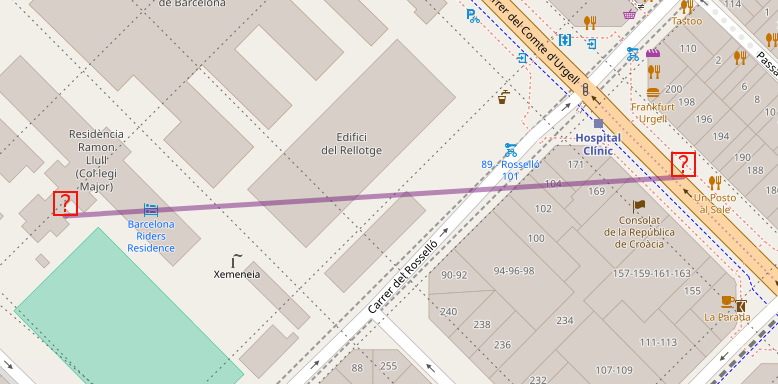
\includegraphics[width=0.7\textwidth]{images/path_map_straight.png}
		\caption{Mapa amb un tram}
	\end{figure}
	
	Si volem unir diferents llocs amb un recorregut no recte, podem afegir punts al traçat marcant els punts de vèrtex sobre el mapa després d'haver marcat el primer \emph{lloc} i tancant el traçat al marcar el segon \emph{lloc}
	
	\begin{figure}[H]
		\centering
		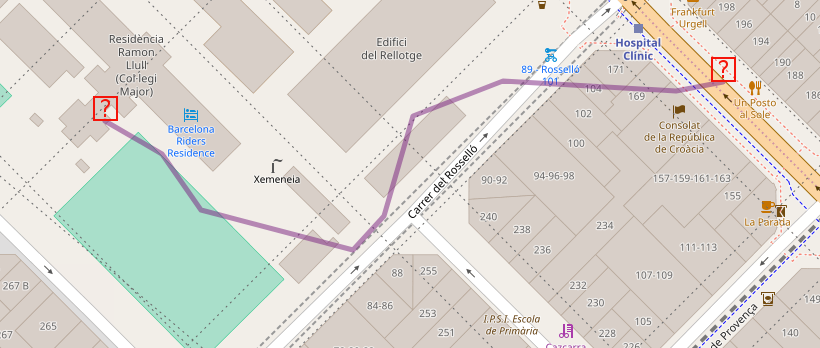
\includegraphics[width=0.7\textwidth]{images/path_map_curve.png}
		\caption{Mapa amb \emph{trams} no rectes}
	\end{figure}

	Per sortir del menú de creació de nous \emph{trams} podem clicar a qualsevol tram existent.
	
	\subsubsection{Edició}
	Per editar un simplement haurem de col·locar el punter a sobre i clicar. Aleshores ens apareixerà un formulari amb tots els atributs que podem alterar.
	
	\begin{figure}[H]
		\centering
		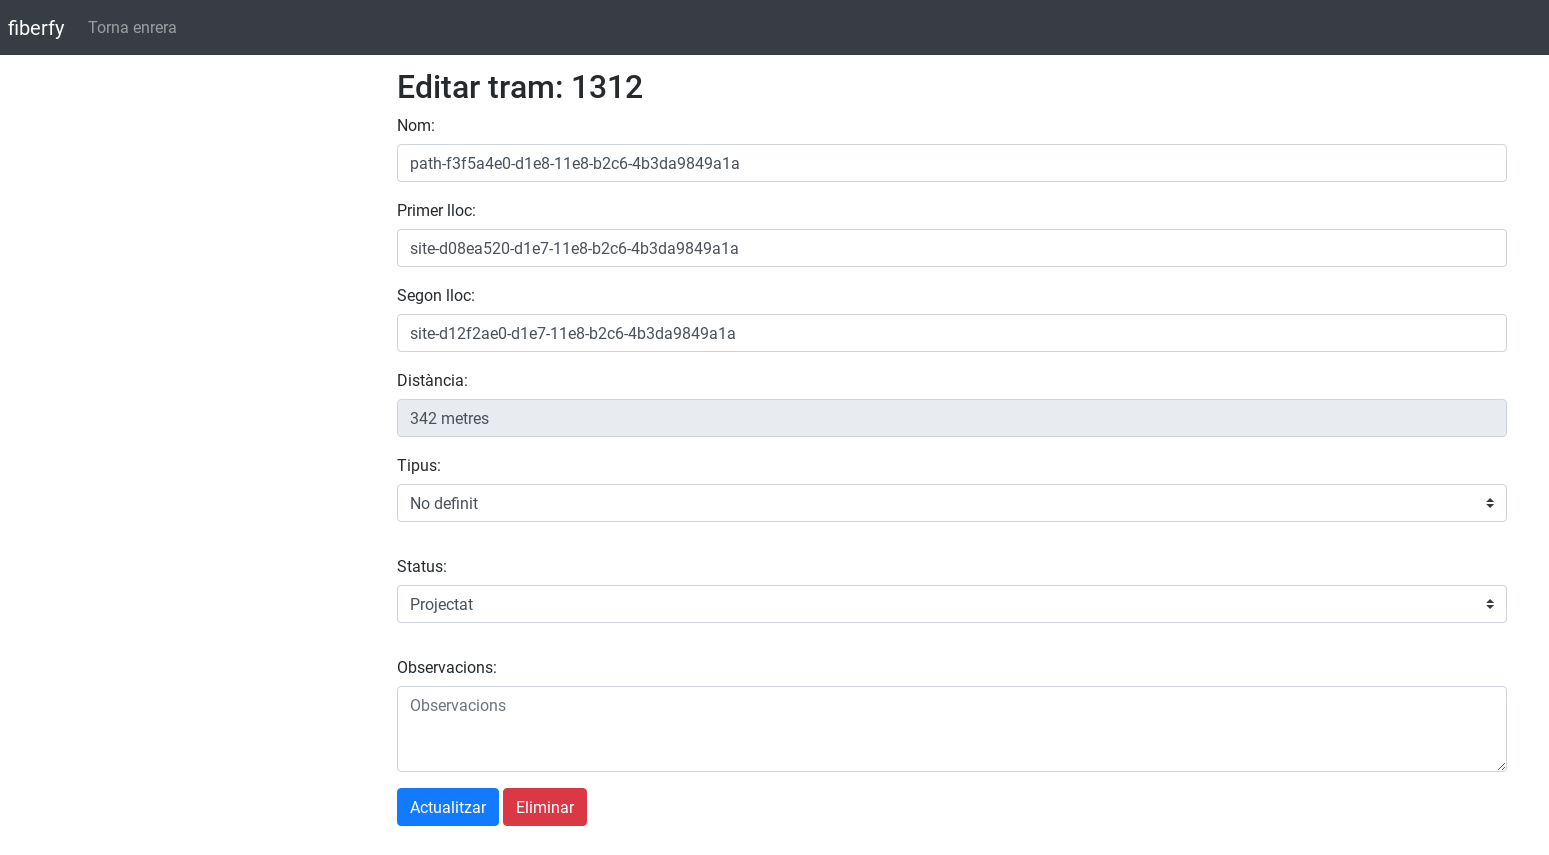
\includegraphics[width=0.8\textwidth]{images/path_edit.png}
		\caption{Formulari d'edició de \emph{trams}}
	\end{figure}
	Aquí podem modificar tots els atributs del tram. En cas de voler alterar el \emph{lloc} d'inici i \emph{lloc} final ens apareixerà un auto-completat que ens permetrà seleccionar entitats de dins del projecte; tot-hi així no se'n recomana el seu ús per evitar possibles desajustos en els camins.
	
	Si hem fet alguna modificació i la volem guardar haurem de clicar el botó \emph{Actualitzar}.
	Si volem eliminar el tram haurem de clicar el botó \emph{Eliminar} i automàticament serem redirigits al mapa.
	
	\newpage
	\section{Cablejat}
	\subsection{Gestió de caixes}
	Les caixes són els elements de telecomunicacions per tal de connectar i distribuir les diferents fibres. Aquests elements són necessaris al inici i final d'una fibra.
	
	\subsubsection{Creació}
	Per tal de crear \emph{caixes} necessitarem haver definit prèviament llocs (d'obra civil). Un cop complert aquest requisit seleccionarem la capa \emph{Xarxa}. Després ja podem clicar qualsevol dels llocs creats anteriorment. Si no contenen \emph{caixes} apareixeran pintats en gris; en cas contrari estaran pintats en taronja. Aleshores s'ens mostrarà el següent formulari:
	
	\begin{figure}[H]
		\centering
		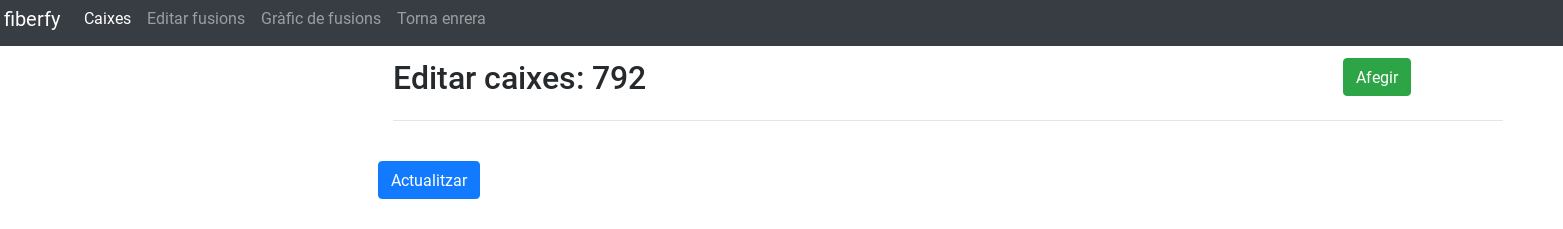
\includegraphics[width=0.8\textwidth]{images/boxes_edit_void.png}
		\caption{Menú de \emph{caixa} buit}
	\end{figure}

	Per tal de seguir amb el procés haurem de prémer el botó verd \emph{Afegir}. Aleshores ja tindrem una \emph{caixa} creada amb la següent aparença:
	
	\begin{figure}[H]
		\centering
		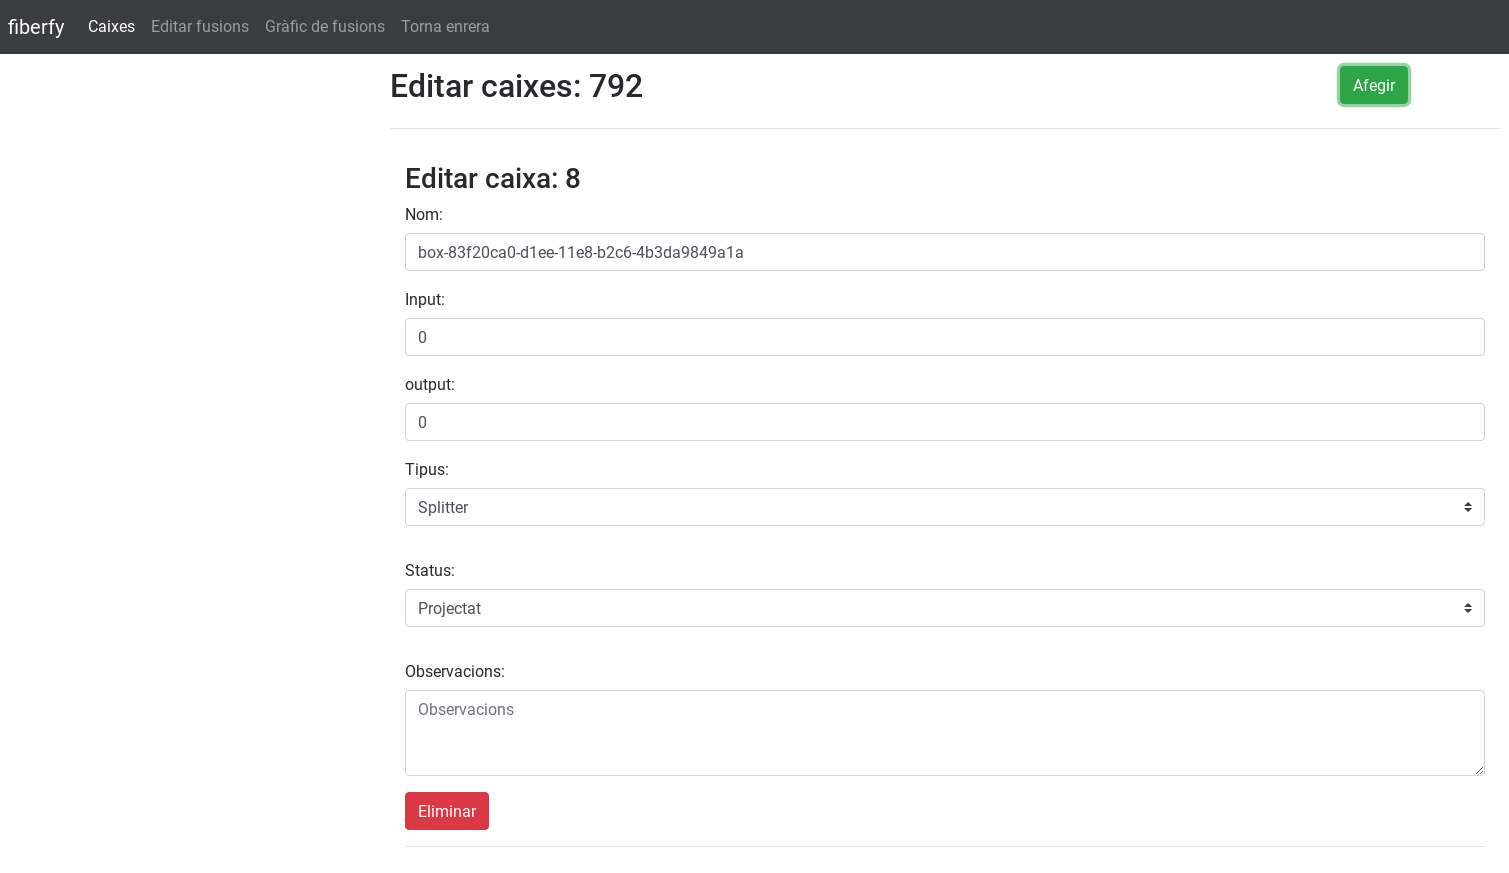
\includegraphics[width=0.8\textwidth]{images/boxes_edit_full.png}
		\caption{Menú de \emph{caixa} omplert}
	\end{figure}

	
	\subsubsection{Edició}
	Per tal de modificar els atributs d'una \emph{caixa} existent només caldrà clicar sobre la capsa en qüestió des de la capa de Xarxa de l'eina. Aleshores ens apareixerà el formulari de creació de \emph{caixes} amb les caixes existents en aquell \emph{lloc}. Per tal de modificar els atributs haurem de validar els canvis utilitzant el botó \emph{Actualitzar} del formulari. Per eliminar caixes haurem de prémer el botó \emph{Eliminar}.
	
	Dins d'aquest formulari també podrem establir el tipus de \emph{caixa} que és i el nombre de fibres d'entrada i sortida que passaran per elles. Aquestes dades seran importants a l'hora de realitzar les fusions de fibres.
	
	\subsection{Gestió de fibres/tubs/cables}
	Un cop les diferents caixes es troben instal·lades ja podem tirar cables amb tubs i fibres.
	
	\subsubsection{Creació}
	Per desplegar fibra entre dos punts del mapa necessitem que aquests estiguin units a través de diferents llocs i \emph{trams} i que continguin almenys una \emph{caixa} a l'inici i al final del recorregut.
	Per començar hem de seleccionar el menú de \emph{Nou Cable} que trobarem al seleccionar la capa de \emph{Xarxa}.
	
	El següent pas serà marcar la primera \emph{caixa} on anirà un dels extrems del cable. Aleshores anirem marcant un a un els llocs per on la fibra anirà passant \footnote{Els extrems sempre han de contenir alguna \emph{caixa}}; el camí que es va fent es mostrarà d'un color vermellós (\emph{trams} i llocs). Un cop acabada la trama de cable per tal de validar-la haurem de clicar una segona vegada sobre l'últim \emph{lloc}.
	
	\begin{figure}[H]
		\centering
		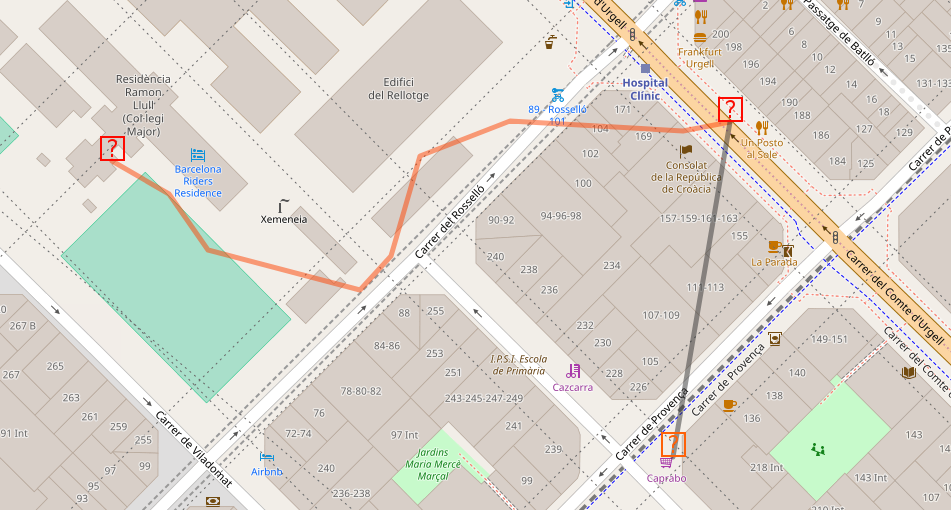
\includegraphics[width=0.7\textwidth]{images/cable_creation.png}
		\caption{Creació de \emph{cables}}
	\end{figure}
	
	\subsubsection{Edició}
	
	Un cop tenim els \emph{cables} creats i sempre des de la capa de \emph{Xarxa}, aleshores podem clicar directament els \emph{trams} que contenen \emph{cables} (sempre de color blau) i ens apareixerà el següent \emph{popup}:
	
	\begin{figure}[H]
		\centering
		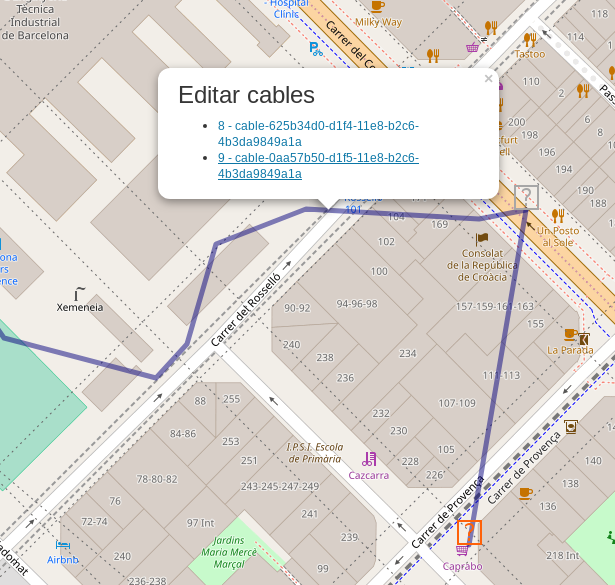
\includegraphics[width=0.7\textwidth]{images/cable_edit_popup.png}
		\caption{\emph{Popup} selecció de \emph{cables}}
	\end{figure}
	
	Un cop seleccionat el \emph{cable} desitjat s'ens mostrarà un formulari com el següent:
	\begin{figure}[H]
		\centering
		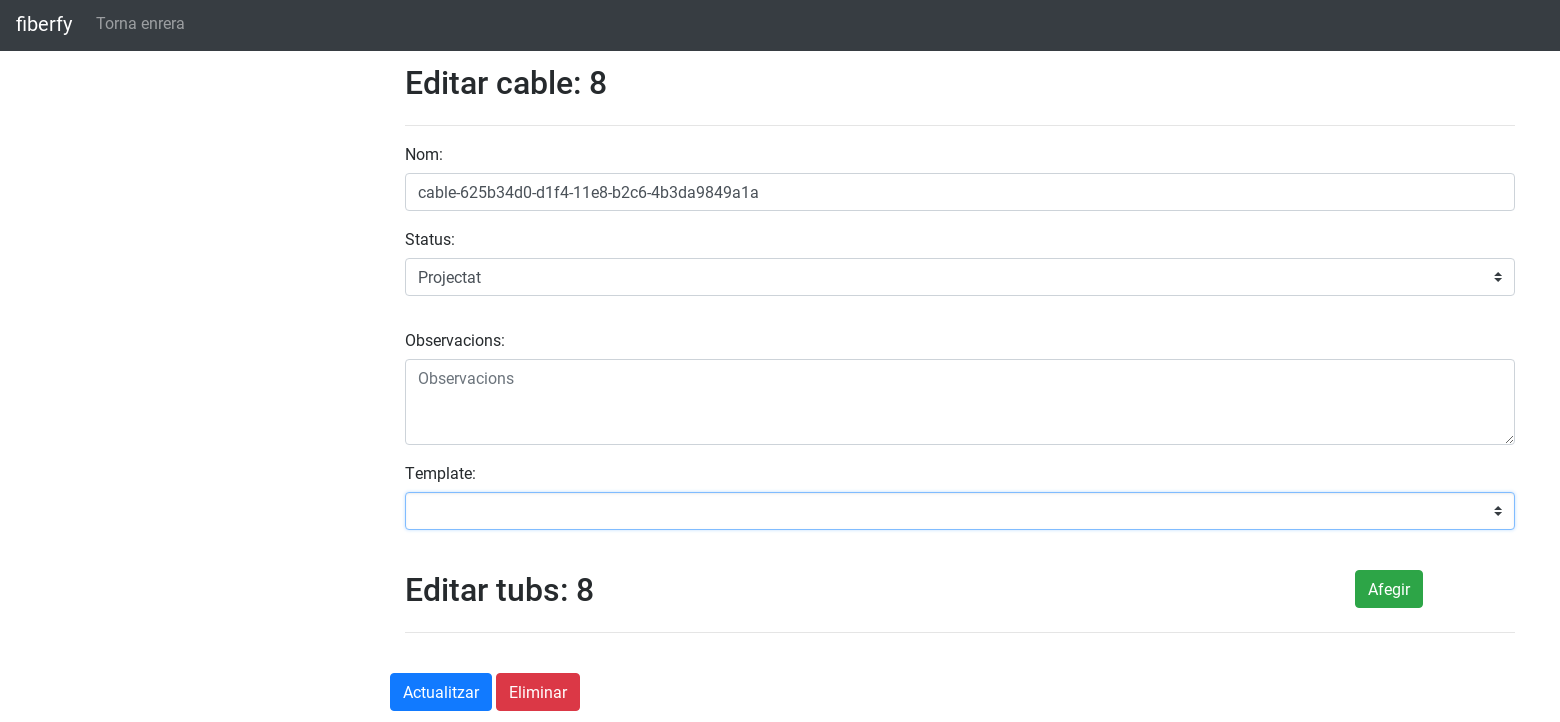
\includegraphics[width=0.8\textwidth]{images/cable_edit_form.png}
		\caption{Formulari d'edició de \emph{cables/tubs/fibres}}
	\end{figure}

	Aquí podrem afegir \emph{tubs} i \emph{fibres} de forma manual (utilitzant els botons d'\emph{Afegir} o seleccionant una plantilla de pre-establerta)
	
	\begin{figure}[H]
		\centering
		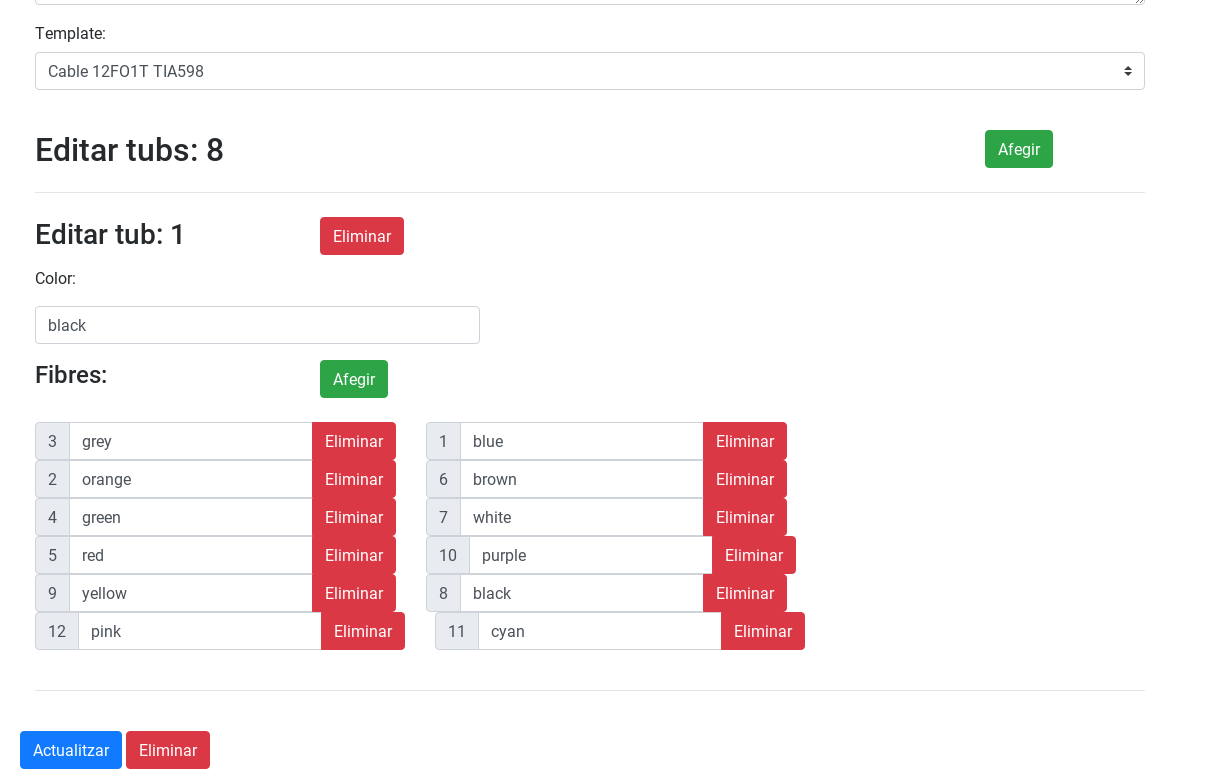
\includegraphics[width=0.8\textwidth]{images/cable_edit_form_template.png}
		\caption{Formulari d'edició de \emph{cables/tubs/fibres} amb plantilla}
	\end{figure}
	
	Per tal de guardar els canvis fets haurem de prémer el botó \emph{Update}. Si volem esborrar \emph{fibres/tubs/cable} haurem de prémer els botons d'\emph{Eliminar}.
	
	\subsection{Gestió de fusions}
	Les fusions són les unions entre diferents fibres d'un cable fibra òptica. Per tal de poder realitzar fusions necessitem com a mínim un cable que contingui fibres tot-hi que el cas d'ús habitual és el d'unir diferents \emph{fibres}.
	
	\subsubsection{Creació i edició}
	Per tal de crear \emph{fusions} entre fibres des de la capa de \emph{Xarxa} hem de prémer el botó d'\emph{Editar Fusions}. Aleshores ens apareixarà un formulari amb un llistat de totes les fibres i les relacions entre elles. Per tal de crear \emph{fusions} simplement hem de seleccionar una \emph{fibra} qualsevol i unir-la amb una altra disponible al desplegable.
	
	\begin{figure}[H]
		\centering
		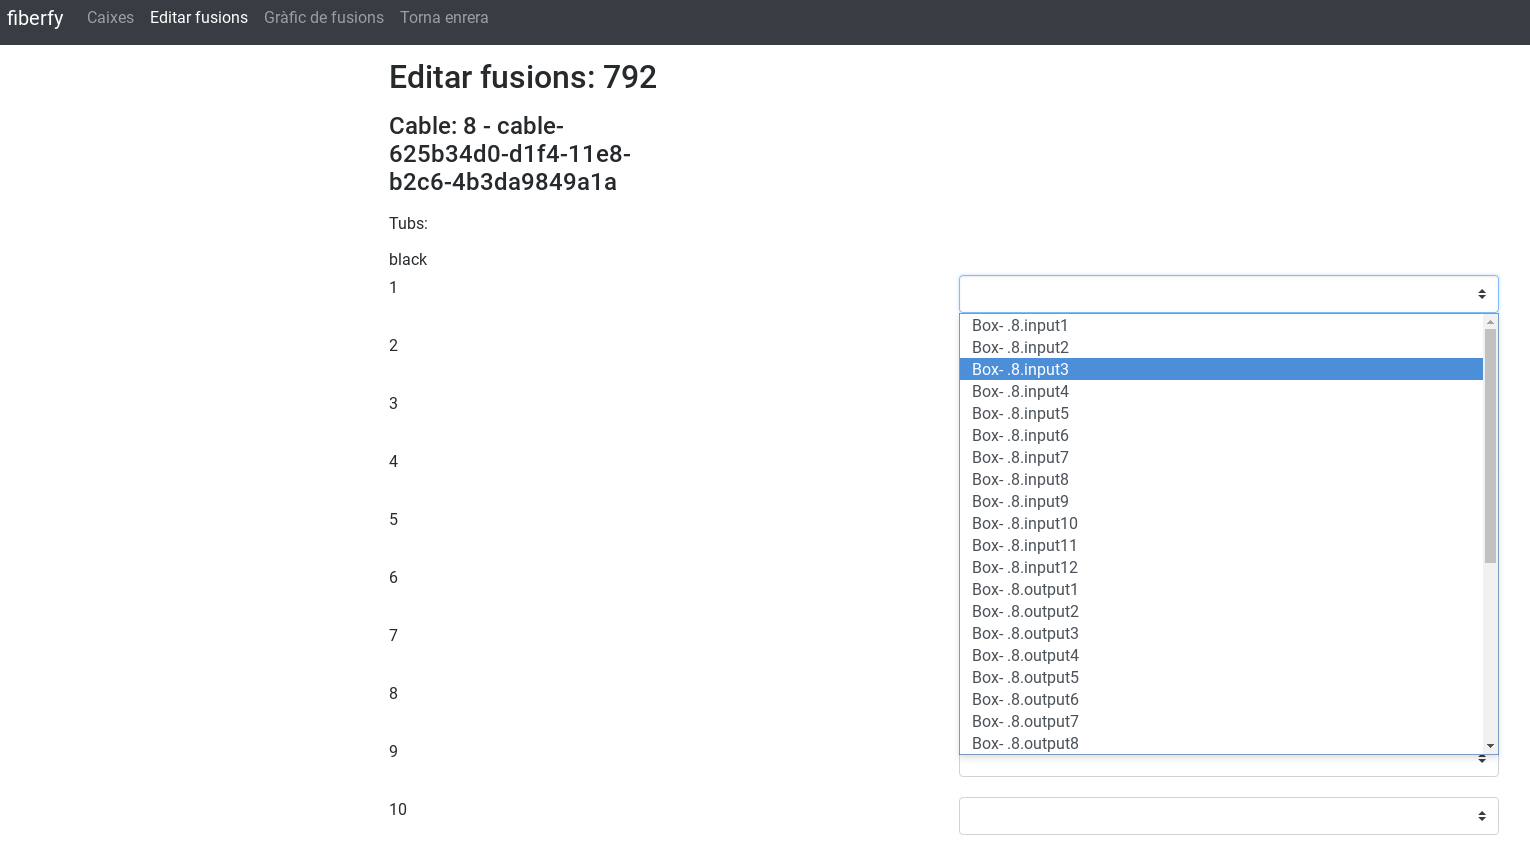
\includegraphics[width=0.8\textwidth]{images/fusions_edit_form_disponible.png}
		\caption{Formulari d'edició de \emph{fusions}}
	\end{figure}

	\begin{figure}[H]
		\centering
		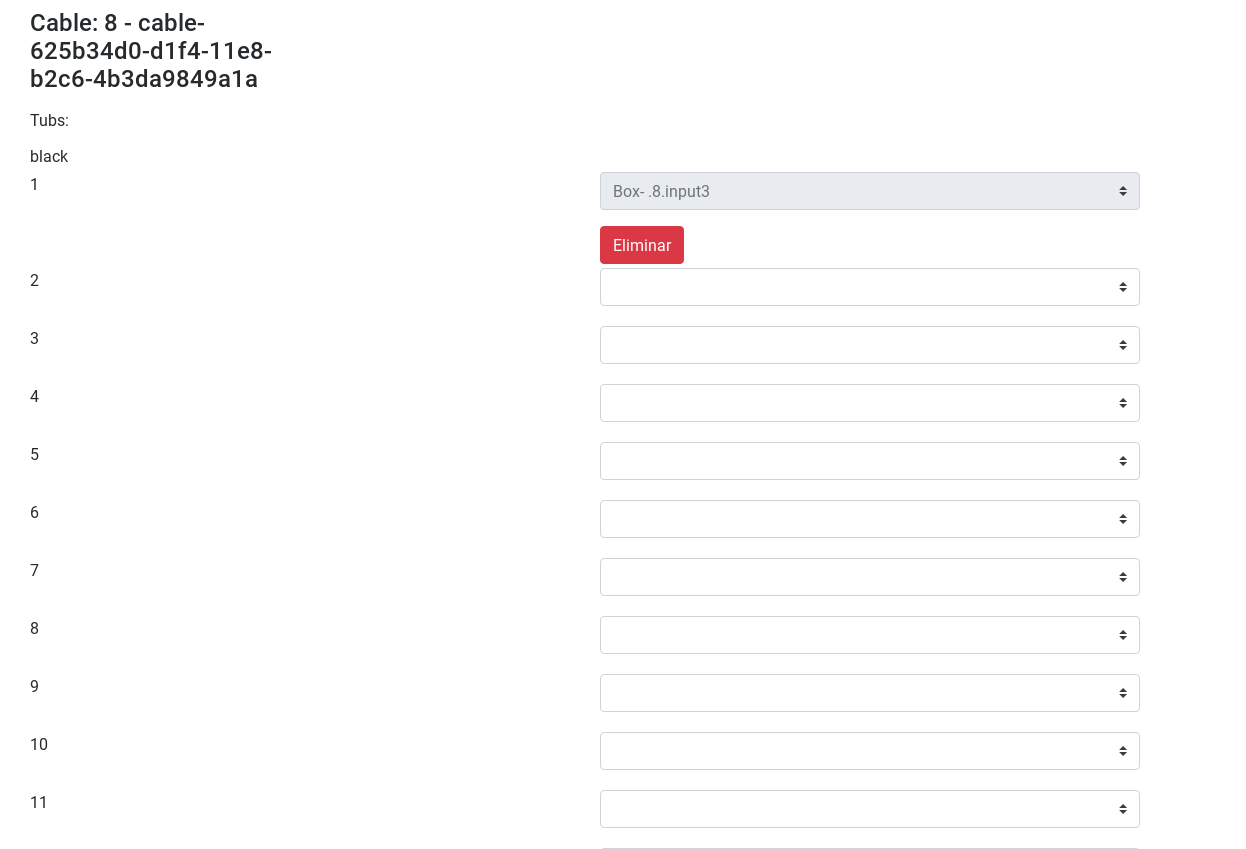
\includegraphics[width=0.8\textwidth]{images/fusions_edit_form_fusion.png}
		\caption{Formulari d'edició de \emph{fusions} amb una fusió}
	\end{figure}

	Aleshores ens apareixerà un formulari que ens indicarà pels diferents llocs quines \emph{fibres} passen. Aquí podrem seleccionar una a una les fibres que volem unir \footnote{A la llista de fibres que apareixerà a cada desplegable, apareixen totes les fibres disponibles i caixes amb (entrades/sortides)}.
	

	\subsubsection{Visualització}
	Per visualitzar les fusions realitzades d'un determinat \emph{lloc} s'ha de clicar el botó \emph{Editar fusions} del menú d'infraestructura de xarxa i després seleccionar la pestanya \emph{Gràfic Fusió} del menú superior. Un cop dins es podran veure les unions dels diferents cables amb el seu color corresponent.
	
	\begin{figure}[H]
		\centering
		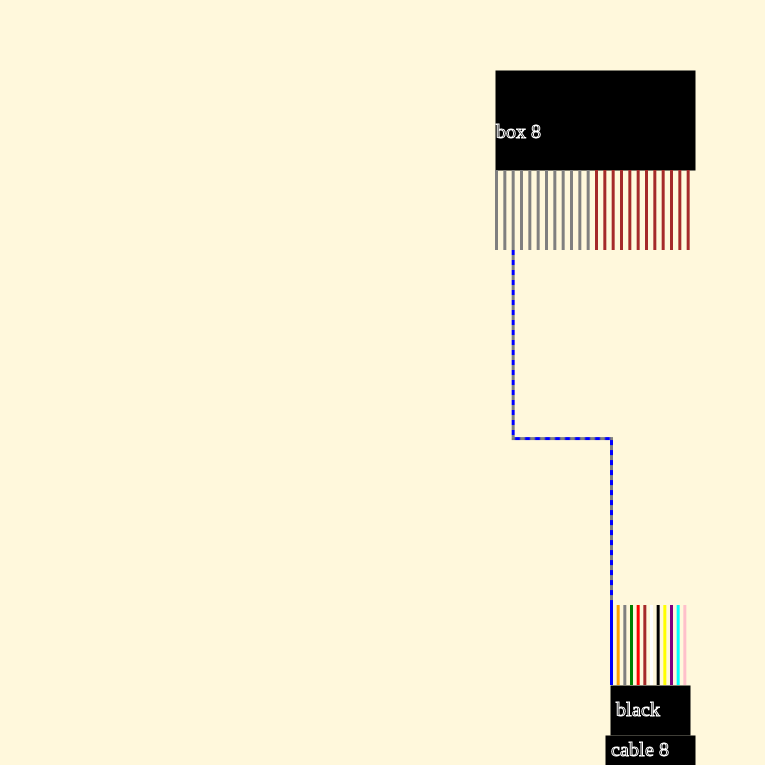
\includegraphics[width=0.7\textwidth]{images/fusions_diagram.png}
		\caption{Visor de \emph{fusions}}
	\end{figure}
\end{document}
